%
% File naacl2019.tex
%
%% Based on the style files for ACL 2018 and NAACL 2018, which were
%% Based on the style files for ACL-2015, with some improvements
%%  taken from the NAACL-2016 style
%% Based on the style files for ACL-2014, which were, in turn,
%% based on ACL-2013, ACL-2012, ACL-2011, ACL-2010, ACL-IJCNLP-2009,
%% EACL-2009, IJCNLP-2008...
%% Based on the style files for EACL 2006 by 
%%e.agirre@ehu.es or Sergi.Balari@uab.es
%% and that of ACL 08 by Joakim Nivre and Noah Smith

\documentclass[11pt,a4paper]{article}
\usepackage[hyperref]{naaclhlt2019}
\usepackage{times}
\usepackage{graphicx}
\usepackage{booktabs}
\usepackage[ruled,vlined]{algorithm2e}
\usepackage{latexsym}
\usepackage{amsmath}
\usepackage{amssymb}
\usepackage{bm}

\newcommand{\rdep}[1]{\ $\xrightarrow{\text{\tiny #1}}$\ }
\newcommand{\speedup}[0]{20X~}
\newcommand{\ahcomment}[1]{\textcolor{blue}{[#1 -AH]}}

\usepackage{url}

%\aclfinalcopy % Uncomment this line for the final submission
%\def\aclpaperid{***} %  Enter the acl Paper ID here

%\setlength\titlebox{5cm}
% You can expand the titlebox if you need extra space
% to show all the authors. Please do not make the titlebox
% smaller than 5cm (the original size); we will check this
% in the camera-ready version and ask you to change it back.

%\hypersetup{draft} % THIS IS NEEDED TO GET IT TO COMPILE. Does not like the tables. AH 11/27

\newcommand\BibTeX{B{\sc ib}\TeX}

\DeclareMathOperator*{\argmaxA}{arg\,max} % Jan Hlavacek

% Extractive sentence compression under lexical and length constraints
\title{Linear Compression under Lexical and Length Constraints}

\author{First Author \\
  Affiliation / Address line 1 \\
  Affiliation / Address line 2 \\
  Affiliation / Address line 3 \\
  {\tt email@domain} \\\And
  Second Author \\
  Affiliation / Address line 1 \\
  Affiliation / Address line 2 \\
  Affiliation / Address line 3 \\
  {\tt email@domain} \\}

\date{}

\begin{document}
\maketitle

\begin{abstract}
Search applications often display shortened sentences which must contain certain query terms and must fit within the space constraints of a user interface. This work introduces a new transition-based sentence compression technique developed for such settings. Our method constructs length and lexically constrained compressions in linear time, by growing a forest in the dependency parse of a sentence. This approach achieves a \speedup speed up over baseline ILP compression techniques, and better reconstructs known-good shortenings under constraints. Such latency gains permit constrained compression of multiple sentences, without unreasonable lag.
\end{abstract}


\section{Introduction}\label{s:intro}

Traditional study of extractive sentence compression seeks to create short, readable, single-sentence summaries which retain the most ``important'' information from source sentences. But search applications often require compressions which must include a user's query terms, and must not exceed some maximum length permitted by screen space.  Figure \ref{f:qf} shows an example.

This study examines the English-language compression problem with such length and lexical requirements. In our constrained compression setting, source sentences $S$ are shortened to compressions $C$ which (1) must include a set of query words $Q$ and (2) must be shorter than or equal in length to a maximum character length, $b \in \mathbb{Z}^{+}$. Formally, constrained compression maps $(S,Q,b) \rightarrow C$, such that $C$ respects $Q$ and $b$.

\begin{figure}[htb!]
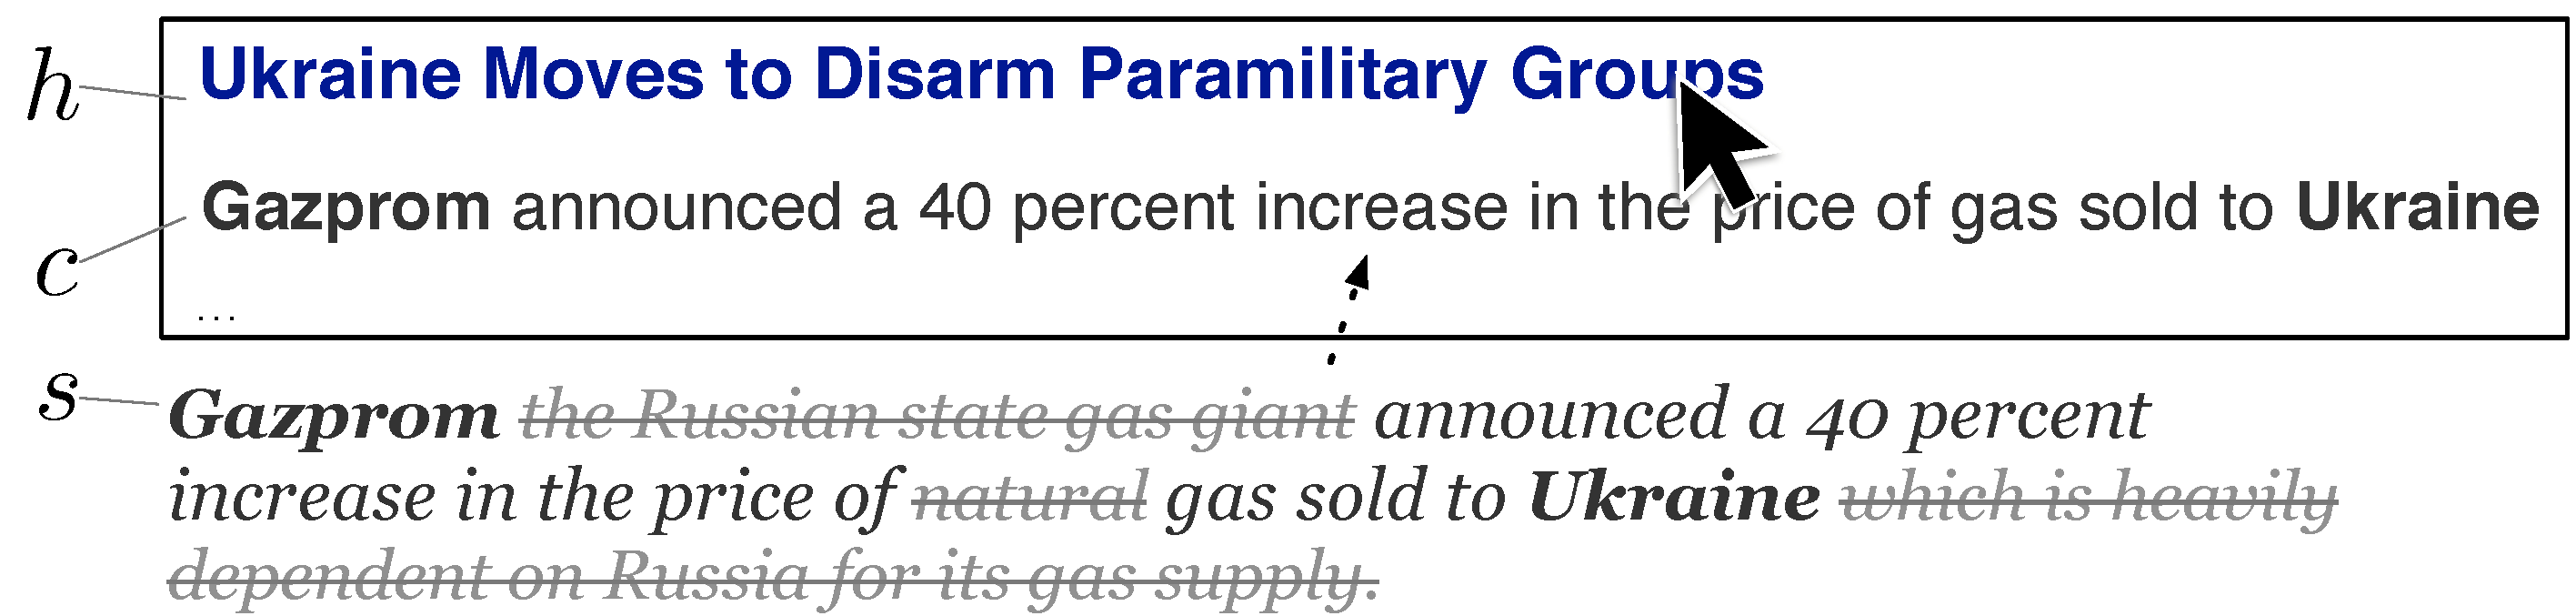
\includegraphics[width=8.5cm]{qf.pdf}
\caption{A search interface (boxed, top) returns a headline $h$ above a constrained compression $C$, shortened from a sentence $S$ in a query-relevant document (italics, bottom). The constrained compression must contain $Q$, the users' query terms (bold), and must not exceed $b=$75 characters in length.}
\label{f:qf}
\end{figure}

Existing compression techniques are poorly suited to this task. While older methods based on integer linear programming (ILP) can trivially accommodate such length and lexical restrictions \cite{clarke2008global,filippova2013overcoming}, these approaches rely on slow third-party solvers to optimize an NP-hard integer linear programming objective\label{s:relatedwork}, requiring user wait time. Meanwhile, newer sequence to sequence methods \cite{filippova2015sentence} do not allow practitioners to specify length or lexical constraints, and require expensive graphics processing units (GPUs) to achieve low runtime latency. These deficits prevent application of existing compression techniques in traditional search engines \cite{hearst2009search}, concept map browsers \cite{falke2017graphdocexplore} and new forms of exploratory textual interfaces \cite{marchionini2006exploratory}, where length, lexical and latency requirements are paramount. 

Thus, in this work, we present a new linear method for constrained compression, which grows a forest in a sentence's dependency parse. We compare this \textit{additive compression} technique to supervised, ILP systems, which also accommodate length and lexical restrictions. Our method has lower theoretical and empirical computational costs, while better reconstructing known-good shortenings. 

\section{Related work}\label{s:relatedwork}


\begin{table}[htb!]
\begin{tabular}{lcc}
\textbf{Approach} & \textbf{Worst-case} & \textbf{Constrained}  \\ \hline
ILP       &   exponential    & yes     \\
LSTM taggers   & linear              & no         \\   
\textbf{Additive} {\small (this work)}  & \textbf{linear}     &      \textbf{yes}   
\end{tabular}
\caption{Supervised ILP compression methods \cite{clarke2008global,filippova2013overcoming,Wang2017CanSH} can easily accommodate length and lexical restrictions, but must solve a known NP-hard problem with worst-case exponential runtime. LSTM taggers \cite{filippova2015sentence} achieve comparable results with linear runtime, but cannot accommodate length or lexical requirements. This work introduces a supervised additive approach (\S\ref{s:system}) which constructs constained compressions in linear time.} 
\label{t:algos}
\end{table}


Extractive compression \cite{Knight2000StatisticsBasedS,clarke2008global,filippova2015sentence,Wang2017CanSH} shortens a sentence by removing tokens, often to aid in a summarization task \cite{Knight2000StatisticsBasedS,almeida2013fast,P16-1188}.\footnote{Some methods shorten sentences via generation instead of deletion \cite{rush2015neural,mallinson18}. Our interest in the extractive setting follows from a motivation to create interpretable,  trustworthy, and practical search systems \cite{Chuang2012InterpretationAT}: users might not trust abstractive summaries \cite{Zhang:2018:MSG:3290265.3274465}, particularly in cases with semantic error.} To our knowledge, this work is the first to consider extractive compression under length and lexical constraints.\footnote{\citet{Li2013DocumentSV} solicit annotations for ``guided'' compression, but do not examine the compression problem under lexical and length constraints.}

Our interest in the constrained compression problem is motivated by search user interfaces \cite{hearst2009search}, which often display query-biased \cite{tombros1998advantages} and length-restricted shortenings.\footnote{Apache Lucene {\small (v7.7)} does not compress sentences to form snippets \cite{lucene}.} 
%\url{https://lucene.apache.org/core/7_5_0/highlighter/index.html}} 
Because such user-facing systems require low-latency \cite{Nielsen,heerschei,Liu2014TheEO}, we adopt a computationally efficient approach. 

We compare our compression method to ILP-based compression techniques \cite{clarke2008global,filippova2008dependency,filippova2013overcoming,Wang2017CanSH}, which can easily accommodate lexical and budget requirements. These methods shorten sentences by optimizing an integer programming objective, a well-known, NP-hard problem \cite{clarke2008global} requiring worst-case exponential computation.\footnote{ILPs are exponential in $|V|$ if when selecting tokens \cite{clarke2008global}, and exponential in $|E|$ when selecting edges \cite{filippova2013overcoming}.} ILP-based techniques typically optimize with an off-the-shelf solver. 

At this time, sequence to sequence sentence compression methods \cite{filippova2015sentence}  cannot enforce lexical or length requirements. This limitation might be reexamined in future work, by modifying or adapting new constrained generation techniques \cite{D16-1140,N18-1119,D18-1443,aaimh}.

\section{Additive compression}\label{s:system}

In this work, we present a new transition-based method for shortening sentences under lexical and length constraints, inspired by similar approaches in transition-based parsing \cite{nivre2003}. We describe our technique as additive compressifon because it constructs a shortening by \textit{growing} a forest in the dependency parse of a sentence. This approach differs from some prior work which
compresses sentences by \textit{pruning} subtrees \cite{Knight2000StatisticsBasedS,berg2011jointly,almeida2013fast,Filippova2015FastKS}. The chief advantage of additive compression is that it can construct constrained compressions in linear time, leading to \speedup lower latency than ILP-based methods (\S\ref{s:autoeval}). 

Additive compression assumes a boolean relevance model: source sentences selected for compression must contain query terms. Many search interfaces (e.g.\ Figure \ref{f:qf}) require such constrained compressions.


\begin{figure}[h]
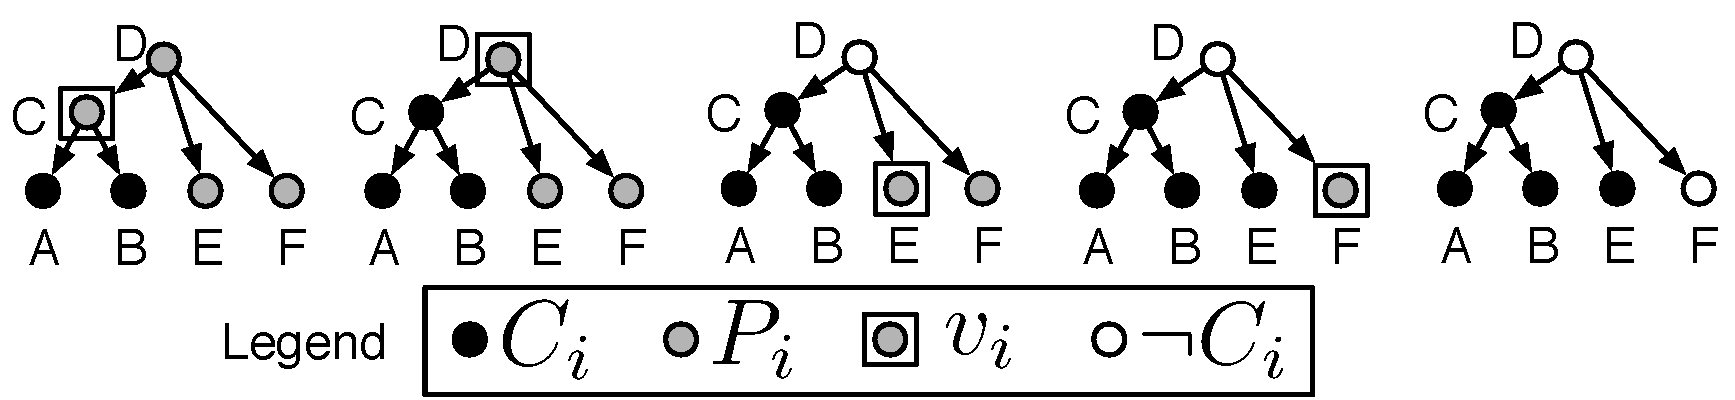
\includegraphics[width=8.2cm]{additive.pdf}
\caption{A stateful procedure (from left to right) produces the final compression $\{$A,C,B,E$\}$. Each candidate $v_i$ is boxed; rejected candidates $\neg C_i$ are unshaded.}
\label{f:walkthru}
\end{figure}

\subsection{Additive procedure}\label{s:formal}

Our method builds a compression by maintaining a state
$(C_i,P_i)$ where $C_i \subseteq S$ is a set of added candidates, $P_i  \subseteq S$ is a priority queue of vertexes, and $i$ indexes a timestep during compression. Figure \ref{f:walkthru} shows a step-by-step example. 

During initialization, we set $C_0 \gets Q$ and $P_0 \gets S \setminus Q$. Then, at each timestep, we pop some candidate $v_i =h(P)$ from the head of $P$ and evaluate $v_i$ for inclusion in $C_i$. (Neighbors of $C_i$ in $P$ get higher priority than non-neighbors in the queue. We break ties in left-to-right order, by sentence position.) If we accept $v_i$, then $C_i \gets C_i \cup v_i$. We discuss acceptance decisions in detail in \S\ref{s:transition}. We continue adding vertexes to $C$ until either $P$ is empty or $C_i$ is $b$ characters long.\footnote{We linearize $C$ by left-to-right vertex position in $S$, which is common for English-language compression.} The appendix includes a formal algorithm. 

Additive compression is linear in the token length of $S$ because we pop and evaluate some vertex from $P$ at each timestep, after $P_0  \gets S \setminus Q$. Additionally, because we never accept $v_i$ if the length of $C_i \cup v_i$ is more than $b$, and because we set $C_0 \gets Q$, our method respects $Q$ and $b$.

\section{Evaluation}\label{s:autoeval}

We compare additive compression to a supervised ILP baseline in terms of latency, readability and token-level F1 score. F1 is the standard automatic evaluation metric for the compression task, used to measure how well each compression method can reconstruct known-good shortenings. Our method achieves higher F1 scores, higher automatic readability scores and \speedup lower latency (Table \ref{t:results}) than ILP techniques. We evaluate the significance of each difference with bootstrap sampling \cite{D12-1091}. All differences are significant {\small $(p < 10^{-2})$}. 

\subsection{Synthetic constrained compression experiment}\label{s:constrained}

In order to evaluate different approaches to constrained compression, we require a dataset of sentences, constraints and known-good shortenings, which respect the constraints. This means we need tuples $(S, Q, b, C_g)$, where $C_g$ is a known-good compression of $S$ which respects $Q$ and $b$ (\S\ref{s:intro}).

To support large-scale automatic evaluation, we reinterpret a standard compression corpus \cite{filippova2013overcoming}
as a collection of input triples and constrained compressions. The original dataset contains pairs of sentences $S$ and compressions $C_g$, generated using headlines. For our experiment, we set $b$ equal to  the character length of $C_g$. We then sample some query set $Q$ from the proper and improper nouns in $C_g$ so that the distribution of cardinalities of queries across our dataset simulates the observed distribution of cardinalities (i.e.\ number of query tokens) in real-world search \cite{Jansen2000RealLR}. Sampled queries are short sets of nouns, such as ``police, Syracuse'', ``NHS'' and ``Hughes, manager, QPR,'' approximating real-world behavior \cite{Barr2008TheLS}.\footnote{See appendix for detailed discussion of query sampling.} 


By sampling queries and defining budgets in this manner, we create {199,152} training tuples and {\ahcomment{TODO}} test tuples, each of the form $(S,Q,b,C_g)$. We re-tokenize, parse and tag the dataset with Stanford CoreNLP 3.8.0 \cite{corenlp}.

\subsection{Implementation: ILP-based compression}\label{s:ilp}

We compare our system to a state-of-the-art, ILP-based method, presented in \citet{filippova2013overcoming}. This approach represents each edge in a syntax tree with a vector of binary features, then learns weights for each feature using a structured perceptron trained on a corpus of sentence--compression pairs. Learned weights are used to compute a global compression objective, subject to structural constraints which ensure the output is a valid tree. This baseline can easily perform constrained compression: at test time, we specify that output must contain $Q$ and respect $b$.

To our knowledge, a public implementation of this method does not exist. We reimplement from scratch using \citet{gurobi}, achieving a test-time, token-level F1 score of  0.690 on the unconstrained compression task, lower than the result reported by the original authors. There are some important differences between our reimplementation and the method reported in \citet{filippova2013overcoming}, largely resulting from differences in syntactic formalisms. We describe these differences in detail in the appendix. Note that our additive method requires $Q$ and $b$, so we can only compare it to the ILP on the \textit{constrained} (rather than traditional) compression task.

\subsection{Implementation: additive compression}\label{s:transition}

Additive compression accepts or rejects some candidate vertex $v_i$ at each timestep $i$. 
We learn such decisions using a corpus of tuples $(S,Q,b,C_g)$ (\S\ref{s:constrained}). Given such a tuple we can construct a unique oracle compression path by $(1)$ initializing $C_0$ with $Q$, $(2)$ choosing $v_i = h(P)$ at each timestep, and $(3)$ adding $v_i$ to $C_i$ iff $v_i \in C_g$. This procedure can reconstruct all $C_g$ in the original \citet{filippova2013overcoming} corpus. 

We use such oracle paths to train a model of oracle inclusion decisions, ${p(y_i  = 1 | v_i, C_i, S_i)}$. We initially experimented with neural techniques, following the \citet{D14-1082} approach to transition-based parsing. But we found that feature-based, binary logistic regression achieved similar performance with much lower latency. This approach is also better suited to applications in fields like social science and journalism, where expensive GPUs are not available. The features in our model fall into 3 classes.

\textbf{Edge features} describe the properties of the edge $(u,v)$ between $v_i \in P$ and $u \in C_i$. We use the feature function from \citet{filippova2013overcoming}, described in detail in the appendix. This allows us to compare the performance of our local additive model with a global ILP objective (Table \ref{t:results}), which uses the same feature set.\footnote{If $v_i$ is disconnected from $C_i$, as in step 3 of Figure \ref{f:walkthru}, the only local feature is the type of the edge governing $v_i$.}

\textbf{Global features} represent the relationship between $v_i$ and the overall compression $C_i$. Overall features include information such as the position of $v_i$ in the sentence, relative to the right-most and left-most vertex in $C_i$, as well as history-based information such as the fraction of the character budget used so far. Such features allow the model to reason about which sort of vertexes should be added to $C$, given $Q$ and $S$. For instance, global features allow the model to learn if the oracle usually adds tokens to the right or left of $C_i$.

\textbf{Interaction features} are formed by crossing all global features with information about if $u$ governs $v_i$, if $v_i$ governs $u$ or if there is no edge $(u,v_i)$ in the parse.

The appendix contains additional details regarding model tuning and implementation. 

\subsection{Implementation: ablations and baselines}
We implement two additional methods, for comparison. We measure performance of a random baseline, which accepts $v_i$ randomly at the marginal training-time acceptance rate. We also implement an additive method, which makes inclusion decisions using just edge features. This ablated method achieves a lower F1 than the ILP (Table \ref{t:results}), which integrates the same information to optimize a global objective. However, adding global features (Table \ref{t:results}, bold) informs local acceptance decisions, raising F1 score. 

\subsection{Importance and readability evaluation}\label{s:readabilityinformativeness}

Researchers often use human judgements of \textit{importance} and \textit{readability} to evaluate compression techniques \cite{Knight2000StatisticsBasedS,filippova2015sentence}. In our setting $Q$ determines the ``important'' information from $S$, so human importance evaluations are inappropriate.

We use the automated SLOR metric \cite{lau2015unsupervised} to check the readability of compressions. SLOR normalizes the probability of a token sequence assigned from a language model, by adjusting for both the probability of the individual unigrams in the sentence and for the sentence length, and is known to correlate with human readability judgements for the compression task \cite{kannConl}.\footnote{Longer sentences are always less probable than shorter sentences; rarer words make a sequence less probable.} Based on SLOR scores, our method might produce slightly more readable compressions (Table \ref{t:results}). The appendix details our implementation of SLOR. 

\subsection{Latency evaluation}\label{s:costs}

Unlike ILPs, our method is linear instead of exponential in the worst-case (\S\ref{s:formal}). We test the real latency advantage from such theoretical gains by measuring the wall clock speed of each technique. We observe a \speedup speedup (Table \ref{t:results}) in mean compression time. The appendix contains additional measurement details.

In user-facing applications such latency gains are non-trivial \cite{Nielsen,heerschei,Liu2014TheEO}: compressing even 10 sentences with an ILP (e.g.\ for 10 query results) would take more than a second, a noticeable lag. %Unlike ILP-based methods (which rely on black-box solvers), our Python 3 implementation could also be sped up by reimplementing in faster languages like Java or C. 

\begin{table}[]
\begin{tabular}{lccc}
\centering
Approach & F1 & SLOR &  ms. / sentence  \\ \hline
Random {\small (lower bound) }&{\small 0.654}&{\small 0.000}&{\small 0.557}\\
ILP&{\small 0.000}&{\small 0.000}&{\small 0.000}\\
Additive {\small (edge only) }&{\small 0.818}&{\small 0.000}&{\small 5.680}\\
\textbf{Additive}&\textbf{\small 0.875}&\textbf{\small 0.000}&\textbf{\small 11.806}\\
\end{tabular}
\caption{Test F1 scores, SLOR scores and average latency (milliseconds per sentence) for the constrained compression task. 
The difference between all metrics is statistically significant {\small $(p < 10^{-2})$}.
\ahcomment{$\sigma$?}}
\label{t:results}
\end{table}

\section{Conclusion}

Search interfaces often require low-latency, query-focused and length-constrained compression. We introduce a new additive technique for such settings, which is much \speedup faster than an ILP baseline, while achieving comparable F1 scores. 

%Finally, some shortened sentences will modify the meaning of a sentence. Identifying such cases is a special case of the unsolved textual entailment problem \cite{snli_bowman,Pavlick2016SoCalledNA,linzencompression}. In the future, we plan to apply entailment research to the compression task.  

% ack => Katie, Javier, NLP reading group! 

%\appendix

\begin{figure*}[htb!]
\centering
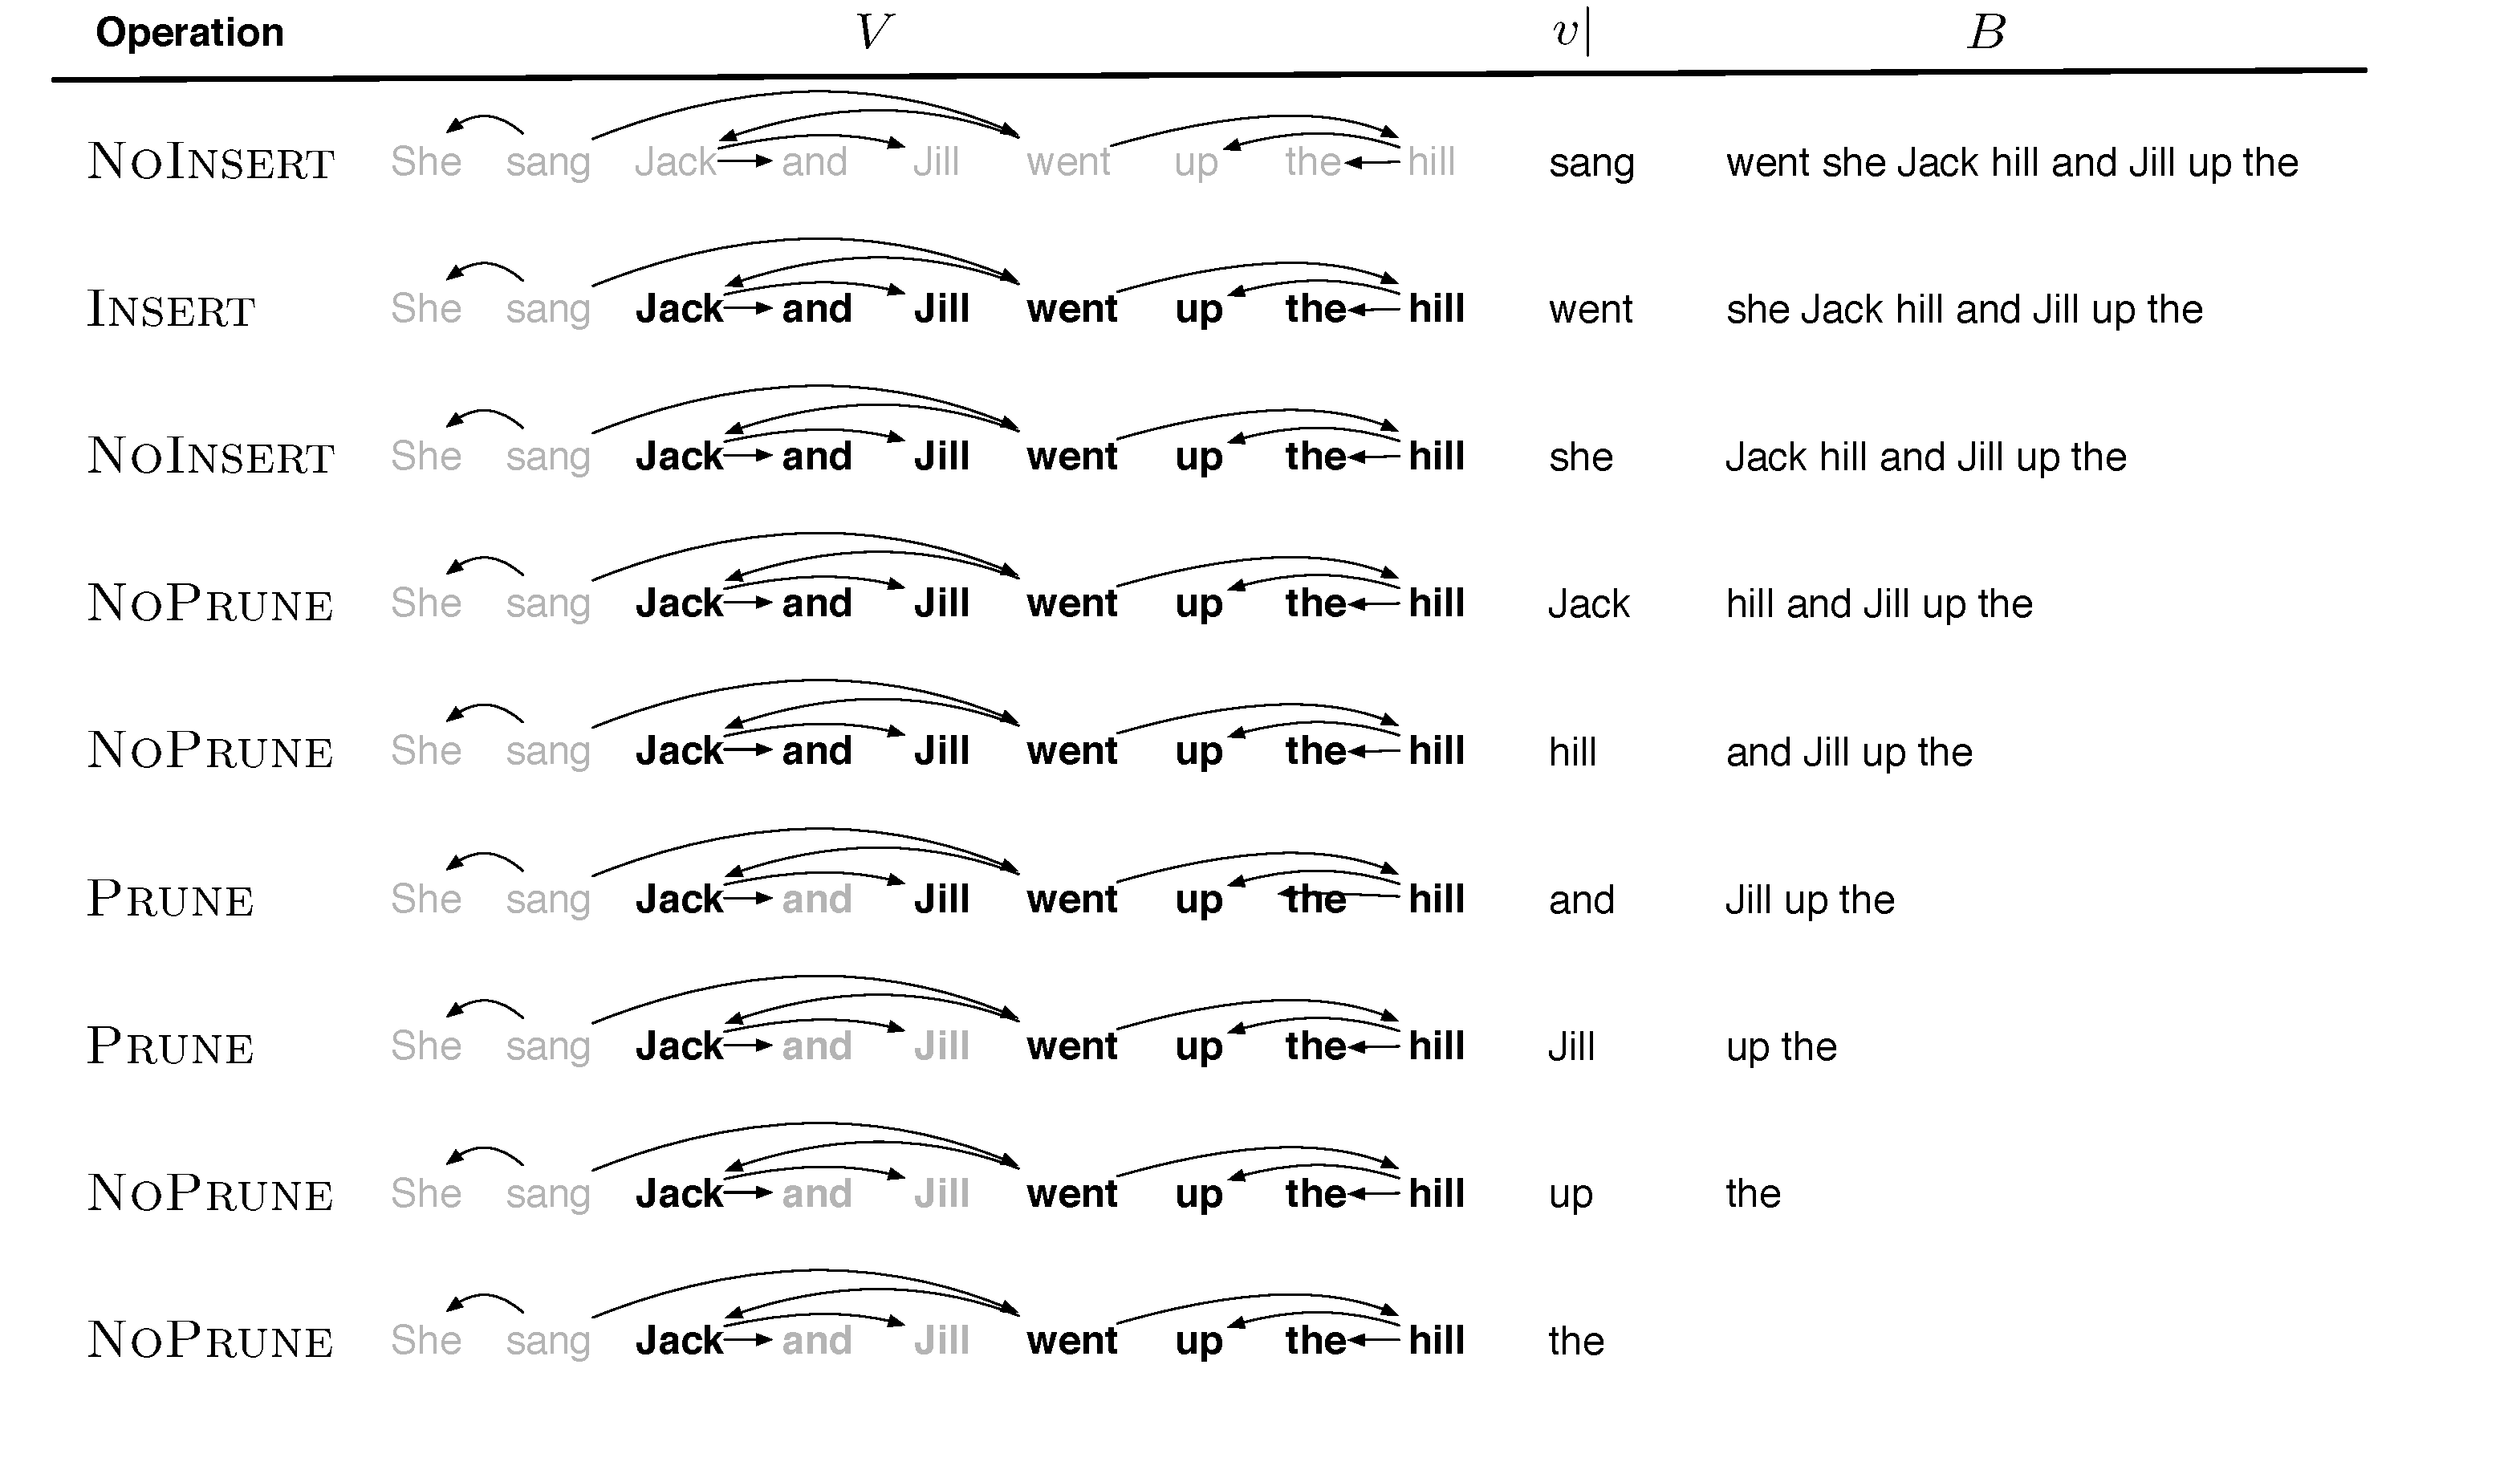
\includegraphics[width=.75\textwidth]{worked.pdf}
\caption{Nine operations of our transition-based compression return the compression: ``Jack went up the hill". At each timestep, the compression has state $(V_j, [v_j|B])$. In the diagram, the tokens in $V_j$ are shown in bold. The token $v_j$ is shown in the third column.}
\label{f:example}
\end{figure*}

\section{Appendix}


\subsection{Reimplementation of \citet{filippova2013overcoming}: additional details}

In this work, we reimplement the method of \citet{filippova2013overcoming}, who in turn implement a method partially described in \citet{filippova2008dependency}.  There are inevitable discrepancies between our implementation and the methods described in these two prior papers.  

Some discrepancies arise from differences in syntactic formalisms. To begin, prior work uses a tree transformation method which is no longer strictly compatible with UD. For instance, the tree transformation from prior work assumes PPs are headed by prepositions, which is not true in UD \cite{Schuster2016EnhancedEU}. We thus reimplement the tree transformation, using the enhanced dependencies representation from CoreNLP, which provides off-the-shelf augmented modifiers and augmented conjuncts that are very similar to the augmented edge labels from prior work. We exclude a syntactic constraint based on the \rdep{sc} relation, which is not included in UD.

Other possible discrepancies arise from differences in part-of-speech taggers. In particular, the aforementioned tree transform from prior work adds an edge between the root node and all verbs in a sentence, as a preprocessing step. This ensures that subclauses can be removed from parse trees, and then merged together to create a compression from different clauses of a sentence. However, we found that replicating this transform literally (i.e. only adding edges from the original root to all ``verbs'') made it impossible for the ILP to recreate some of the gold compressions in the dataset. (We suspect that this is because our part-of-speech tagger and the original part-of-speech tagger employed in \citet{filippova2013overcoming} sometimes return different part-of-speech tags). Our tree transform therefore adds an edge between the root node and \textit{all} tokens in a sentence. With this change, it is always possible for the ILP to output the gold compression.

We use \citet{gurobi} (v7) to solve the liner program. \citet{filippova2008dependency} report using LPsolve.\footnote{\url{http://
sourceforge.net/projects/lpsolve}}  We found that Gurobi sometimes segfaults nondeterminsitically during training. We implement checkpoints which save and restore the state of computation, allowing us to resume training when such errors occur.  We assess convergence by examining the validation F1 score on the constrained task after each pass through the training data. The F1 score increases for each of eight passes through the training data, and then decreases slightly (drops by $10^{-3}$ points). We terminate training at this point. 

Lastly, in Table 1 of their original paper, \citet{filippova2013overcoming} provide an overview of the syntactic, structural, semantic and lexical features in their model. We implement every feature explicitly described in their work, except where otherwise noted (e.g. syntactic feature not compatible with UD). However, additional features included in their model (but not explicity described in print) almost certainly affect performance. 

\subsection{Implementation of SLOR: additional details}

We use the SLOR function to measure the readability of the shortened sentences produced by each compression system. Following \cite{lau2015unsupervised}, we define the function as 

\begin{equation}
\text{SLOR}=\frac{\text{log}P_m(\xi) - \text{log}P_u(\xi)}{|\xi|}
\end{equation}

where $\xi$ is a sequence of words, $P_u(\xi)$ is the unigram probability of this sequence of words and $P_m(\xi)$ is the probability of the sequence, assigned by a language model.  $|\xi|$ is the length (in tokens) of the sentence.

We use a 3-gram language model trained on the \citet{filippova2013overcoming} corpus. We implement with KenLM \cite{Heafield-kenlm}.

\subsection{Subtree and compression brackets: additional details}\label{s:subtree}

Our markup input to our LSTM, $\bm{x}_j$, includes \textbf{subtree brackets} with a complex structure, used to represent the start and end of the tokens which will be pruned or inserted by an operation $o_j \in \{ \textsc{Prune},\textsc{Insert}\}$. The start and end tags are each formed by concatenating two symbols: (1) a symbol $o_j$ indicating the type of the operation proposal (i.e. prune or insert) and (2) a symbol $d$ indicating the dependency type governing $T(v)$, such as \texttt{dobj}. 

Additionally, the markup includes \textbf{compression brackets} which show the extent of the current compression (if the operation is \textsc{Prune}) or the extent of the compression which would result if the operation were to be accepted (if the operation is \textsc{Insert}). Concretely, these brackets show the extent of \textsc{Max}($V_{j+1}, V_{j}$) within $s$ where, \textsc{Max} selects the largest set by cardinality and where $V_{j+1}$ is all tokens which would be in $V$ at step $j+1$, if the system were to execute operation $o$ at timestep $j$. If $o_j=\textsc{Prune}$ then $V_{j+1}$ will be smaller than $V_j$ and the bracket symbols will show the extent of the current $V_j$. If $o_j=\textsc{Insert}$, then $V_{j+1}$ will be larger than $V_j$ and the compression brackets will show the extent of the compression which would result if the tokens were to be inserted. 

\subsection{Neural net training: additional details}

We note several additional details about our neural network training procedure, including hyperparameter settings.


\begin{table}[htb!]
\begin{tabular}{@{}ll@{}}
\toprule
Batch size         & 135                      \\ 
Hidden size        & 907                        \\
Embeddings dim.    & 300                      \\
Total fully-connected layers & 2                        \\
Fully-connected layers, hidden sizes & $(92, 2)$ \\
Fully-connected layers, dropout & $(0.309, 0.408)$ \\
Fully-connected layers, activations        & Relu, Linear             \\
Learning rate      & $4.593 * 10^{-4}$   \\
Weight decay       & $2.421 * 10^{-8}$   \\ \bottomrule
\end{tabular}
\caption{The hyperparameters for our model. The learning rate and weight decay parameter each clearly affect validation accuracy. The importance of other parameters is less clear. } 
\end{table}

\begin{itemize}
\item{We train on 8 million tuples. The cardinality of the training set was bounded by available hardware resources, not by the total number of oracle tuples which can be generated with the \citet{filippova2013overcoming} dataset.}
\item{We weight each training instance $(\bm{x_j}, y_j)$ using the default class weighting scheme in Scikit-learn \cite{Pedregosa:2011:SML:1953048.2078195}. The formula for assigning weights is $\frac{T_o}{2 * T_{o,j}}$. $T_o$ is the total number of training examples of accepted and rejected instances of the operation proposal $o$ (e.g. $T_o$ = total number of \textsc{Prune} examples + total number of \textsc{NoPrune} examples). $T_{o,j}$ is the total number of training operations labeled $y_j$ for operations of proposal type $o$ (e.g. $T_{o,j}$ = the total \textsc{NoPrune} operations, if $y_j=0$ and $o$ = \textsc{Prune}). The 2 in the numerator denotes the total number of classes. Alternative weighting methods are left for future work.}
\item{We experimented with ELMo vectors \cite{Peters:2018}, but found that we were able to achieve similar validation accuracies with much smaller embeddings. It is possible that ELMo-like vectors could be used to increase performance in the future.}
\end{itemize}

\bibliography{abe}
\bibliographystyle{acl_natbib}

\bibliography{abe}
\bibliographystyle{acl_natbib}

\end{document}